\documentclass[12pt,a4paper,twoside]{report}
\usepackage[T1]{fontenc}
\PassOptionsToPackage{defaults=hu-min}{magyar.ldf}
\usepackage{fancyhdr}
\usepackage[magyar]{babel}
\usepackage{listings}
\usepackage{xcolor}
\usepackage{caption}
\usepackage{graphicx}
\usepackage{amsthm}
\usepackage{amsmath}
\usepackage{amssymb}
\usepackage[utf8]{inputenc}
\usepackage{graphicx}
\theoremstyle{definition}
\DeclareMathOperator{\tg}{tg}
\newtheorem{definicio}{Definíció}[chapter]

\renewcommand{\lstlistingname}{kód}
\lstset{
inputencoding=utf8/latin2,
language={Python},
basicstyle=\footnotesize,
numbers=left,
breaklines,
postbreak=\hbox{$\color{red}\hookrightarrow\ $},
keywordstyle=\bfseries\color{blue},
}

\footnotestyle{rule=fourth}

\begin{document}

%! this is kinda not what has to be here, rework
\pagestyle{fancy}
\fancyhf{}
\fancyhead[EL]{\thepage}
\fancyhead[ER]{\nouppercase{\small\sffamily\leftmark}}
\fancyhead[OR]{\thepage}
\fancyhead[OL]{\nouppercase{\small\sffamily\rightmark}}

\title{\textsc{Assassin's Creed Reneszánsz}}
	\author{Lovász Ákos\\Programtervező Informatikus}
	\date{\today}
	\maketitle
	\tableofcontents

\chapter{urmoms}
\section{the start}
Fent, a magasban fáklyák lobogtak, és fénybe borították a Palazzo Vecchio és Bargello tornyait, de valamivel északabbra, a katedrális előtti téren csupán néhány lámpás pislákolt. Ezek némelyike gyengén megvilágította az Arno folyó rakpartját is, ahol a sötétség közeledte még fenyegetőbb volt; az itteni városlakók jónak látták idejekorán nyugovóra  térni  házuk  oltalmában. 
\section{the middle}
A homályban  már  csak  néhol mozgott  egy-egy  alak:  \emph{matrózok,  akik  kapkodva  tekerték  össze  a öteleket,}  és  súrolták  a  fedélzetet,  miután  befejezték  az  utolsó javításokat hajójuk vitorlázatán, kikötőmunkások, akik sietve hordták a rakományukat a közeli 
\subsection{raktár}
raktárak biztonságot adó falai közé. Bár az utcák néptelenek voltak, azért az éjszakában ide is jutott némi fény a kocsmák és bordélyházak ablakaiból.
\Az{\pageref{abra-raid}}.~Oldalon található \ref{abra-raid}.~kép teljesíti a valahanyas követelményt\footnote{Ezt ne hagyd bent prod-ban, meg legyen 12es req. compliant}

\begin{figure}[th!]
    \centering
    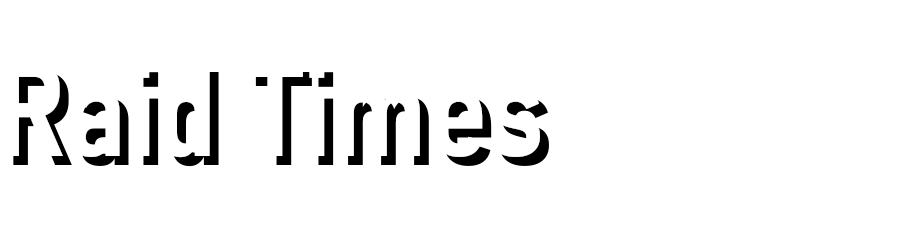
\includegraphics[width=4cm]{raid.png}
    \caption{Raid header}
    \label{abra-raid}
\end{figure}
%* This completes requirement 13.
\begin{itemize}
    \item De  tudta, ez alkalommal túl messzire  ment. Vieri arca bíborvörösre változott a dühtől. 
    \begin{enumerate}
        \item Elég volt, Ezio, te ócska szájhős! Lássuk, a kardodat is olyan jól 
        forgatod-e, mint a nyelved!
        \begin{itemize}
            \item Öljétek le a fattyúkat! - üvöltötte.
        \end{itemize}
    \end{enumerate}
\end{itemize}

\begin{table}[th!]
    \centering
    \begin{tabular}{c|c|c}
        \hline
        111&222&333\\
        \hline
        aaa&bbb&ccc\\
        \hline
    \end{tabular}
    \caption{PLDAUL}
    \label{tablazatom}
\end{table}

Ekkor  újabb  kődarab  süvített  át  a  levegőn,  de  ezúttal  nem 
kihívásnak  szánták.  Oldalról  találta  homlokon  Eziót,  akinek 
felszakadt  bőre  alól  vér  buggyant  elő.  Ezio  egy  pillanatra 
hátratántorodott, amint Vieri bandája kőzáport zúdított rá. Emberei is 
épphogy csak magukhoz tértek, mire a Pazzi-banda lefutott a hídról, 
és rárontott Ezióra és csapatára. A támadás olyan gyors volt, hogy 
azonnal közelharccá fajult, mivel még arra is alig lett volna idő, hogy 
kardot  vagy  akár  tőrt  rántsanak,  így  a  két  csoport  eleinte  puszta 
kézzel ment birokra. 
Az összecsapás vad és brutális volt – a kőkemény rúgásokat és 
ádáz ökölcsapásokat a repedő csontok hátborzongató hangja kísérte. 
Egy darabig megjósolhatatlan volt a harc kimenetele, aztán Ezio, aki 
a  szemébe  csorgó  vértől  már  alig  látott,  észrevette,  hogy  legjobb 
emberei közül kettő a földre bukik, és összegörnyed az őket taposó 
talpak alatt. Ekkor közvetlen közelről felhangzott Vieri kacaja, aki 
egy kővel a kezében végzetes csapásra lendítette karját Ezio feje felé. 
Ezio  ösztönösen  elhajolt,  de  hiába  védte  ki  a  széles  ütést,  a 
lendülettől  a  földre  zuhant.  Az  Auditore-tábor  lassan,  de  biztosan 
kezdett  alulmaradni.  Mielőtt  újra  lábra  állt,  Eziónak  sikerült 
szabaddá  tennie  tőrét,  és  vaktában  kaszabolva  szerencsésen 
belevágnia egy keménvkötésű Pazzi-orgyilkosba, aki kivont tőrrel és 
karddal készült lemészárolni őt. Ezio tőre a combján érte a támadót, 
átszakítva  a  ruhaszövetet,  az  izmokat  és  az  inakat.  Ellenfeléből 
velőtrázó  üvöltés  szakadt  fel,  eldobta  fegyvereit,  kezét  a  sebére 
szorította,  melyből  bőven  bugyogott  a  vér,  majd  tehetetlenül 
előrebukott. 
Amikor Ezio végül feltápászkodott és körbenézett, azt látta, hogy a 
rivális banda bekerítette valamennyi emberét, és fokozatosan szorítja 
őket a templom fala felé. Érezte, hogy az erő kezd visszatérni lábába, 
és  nekilátott  utat  törni  a  társaihoz.

Lasd \az{\ref{abra-raid}}.~tablazatban a dolgot amit latnod kell
\chapter{urdads}
\section{urgrandmas}
Aznap  a  Hold  magasra  kúszott  fel  az  égen,  hogy  fölényes 
díszszemlét tartson a csillagok miriádnyi serege felett. Fénye ezüstre 
festette  azt  a  nyílt  terecskét  is,  ahol  a  Ponte  Vecchio 
belekapaszkodott a folyó északi partjába. 
\subsection{a hid}
A hídra épült házak boltjai, 
melyeket napközben elárasztott a nyüzsgő tömeg, most sötétek és 
némák voltak. A holdfény egy feketébe öltözött alak körvonalait is 
kirajzolta, aki a Santo Stefano al Ponte templom tetején állt. Egy 
magas és büszke fiatalemberét, aki alig töltötte be tizenhetedik évét. 
Miközben  elmélyülten  vizsgálta  az  alatta  elterülő  teret,  kezét 
szájához  emelte,  és  halk,  de  átható  füttyjelet  hallatott.  Azonnal 
észrevette, hogy válaszul először egy, majd három, aztán egy tucat, 
végül vagy húsz férfi lépett ki a térre a sötét utcákból és az épületek 
boltívei alól. 
\subsection{sokan}
Valamennyien fiatalok voltak, mint ő, övükben kard és 
tőr,  legtöbbjük  feketébe  öltözve,  némelyik  vérvörös,  zöld  vagy 
azúrkék  csuklyát,  kalapot  viselt.  A  vészjósló  külsejű  ifjoncok 
csoportja legyező alakban szétnyílt, mozgásuk kihívóan büszke volt. 

\begin{definicio}\label{definicio}
    anyad se szeret
\end{definicio}

\section{urgrandpas}
A  fiatalember  lenézett a halvány  fényben úszó, elszánt arcokra, 
melyek  egytől  egyig  rászegeződtek,  és  feje  fölé  emelt  öklével 
konokul tisztelgett nekik. 

\section{program}
tedd ide a forraskod.py-t

\end{document}

%?1. A forrásfájl csak billentyűzetről begépelhető karaktereket tartalmaz-zon. Minden más karaktert LATEX-parancsokkal illetve ligatúrákkal adjon meg (pl. ,, ''-- \dots \"{e}).

%?2. Az oldaltörések legyenek automatikusak, ne használjon \newpage illetve \pagebreak vagy ezekhez hasonló parancsokat.

%?3. Ne legyenek sorvégi túlcsordulások. Ellenkező esetben a naplóban az„Overfull \hbox in paragraph” üzenet olvasható. A megszüntetésüketaz optimális tördelés miatt mindig átfogalmazással érje el, ne használjon \sloppy vagy \linebreak parancsokat

%*4. Használjon report osztályt. Az oldalméret legyen A4, az alapbetűméret 12 pt, a nyomtatott verzió kétoldalas.

%*5. A dokumentum főszövege legyen magyar nyelvű. A magyar.ldf legyendefaults=hu-min opcióval betöltve. Ügyeljen rá, hogy T1 belső kódo-lást használjon. 

%*6. A lábjegyzetek felett legyen vonal, melynek hossza a szövegtükör szé-lességének negyede.

%*7. Definiáljon az amsthm csomag segítségével egy definicio nevű számozott tételszerű környezetet definition stílussal, melynek címe „Definíció”, a számlálóőse pedig a fejezet (chapter) száma. 

%!8. Állítsa be a fej- és láblécet a fancyhdr csomaggal a következők szerint:a) A fancyhdr csomagot úgy töltse be, hogy a szintinformációk magyar tipográfiával jelenjenek meg (azaz még a babel előtt). 3 pontb) Fejezetnyitó oldalon a fejléc üres, a lábléc közepén az oldalszámnormál betűvel és mérettel áll (azaz ne definiálja át a plain stí-lust). 1 pontc) Nem fejezetnyitó páros oldalon a fejléc bal felén az oldalszámnormál betűvel és mérettel, míg jobb felén a fejezetinformáció(\leftmark) groteszk betűtípussal (\sffamily) small (\small)méretben áll. 1 pontd) Nem fejezetnyitó páratlan oldalon a fejléc jobb felén az oldalszámnormál betűvel és mérettel, míg bal felén a szakaszinformáció(\rightmark) groteszk betűtípussal (\sffamily) small (\small méretben áll. 1 ponte) A fejlécnél legyen lénia, de a láblécnél n(ez a fancyhdr alapbe-állítása).

%*9. A címoldal tartalmazza a címet, szerzőt, szakot és a dokumentum fordításának dátumát (pontosabban bármelyik fordításnál az aktuális dátum jelenjen meg, ami az alapbeállítás). 

%*10. A címoldal után álljon tartalomjegyzék. 

%?11. A szöveg álljon legalább két számozott fejezetből, fejezetenként legyenlegalább két számozott szakasz. Minden fejezet legyen legalább háromoldal. A főszöveg legyen sorkizárt (ami alapbeállítás). Egy szakaszonbelül legyen több bekezdés. Értelmes legyen a szöveg, ne használjon lorem ipsumhoz hasonló megoldást. 

%?12. Illesszen be egy 5 cm széles képet (jpg, png, pdf) úsztatott környezetben, középre igazítva, számozással, felirattal. 

%*13 A szövegben legyen három szint mélységű lista.

%!14. Használja a definicio környezetet és hivatkozzon rá. A hivatkozásnál használjon automatikus határozott névelőt. 

%!15. Hivatkozzon a 2. fejezetre és annak nyitó oldalszámára. Mindkét hivatkozás előtt álljon automatikus határozott névelő.

%?16. Írjon néhány lábjegyzetet. Ügyeljen arra, hogy a lábjegyzet jelölője előtt nincs szóköz, továbbá a szöveg egész mondatokból áll.

%!17. Használjon idézőjelet és gondolatjelet. A gondolatjel valóban gondolatjel szerepkörben legyen, ne csak nagykötőjelként.

%!18. Az alábbi képletet írja le kiemelt számozott matematikai környezetben.𝑔: R∖{𝑛𝜋 : 𝑛 ∈Z}→R, 𝑔(𝑥) :=⎧⎨⎩ctg3(𝑥) sin(2𝑥)𝑥−1 , ha 𝑥 > 1,𝑥(︁𝑥22 + 1)︁, különben. A képletszámra hivatkozzon. A ctg operátorjelet a preambulumbandefiniálja. Nem baj, ha a képlet nem illeszkedik a témába. 

%!19. Jelenítsen meg egy programkódot a listings csomaggal. A sorok legyenek számozva. A programkód ne a tex fájlban legyen begépelve,töltse be külön fájlból. A programkód kulcsszavai és megjegyzései le-gyenek kiemelve. Nem baj, ha a kód nem illeszkedik a témába. 

%!20. A végén legyen irodalomjegyzék thebibliography környezettel. A bibliográfiai elemek legyenek számozottak. A főszövegben hivatkozzon azirodalomjegyzék egy elemének egy adott oldalára \cite paranccsal.Az oldal a \cite opciójában legyen megadva. 